% REMEMBER: You must not plagiarise anything in your report. Be extremely careful.

\documentclass{l4proj}

    
%
% put any additional packages here
%
\usepackage{forest}

\begin{document}

%==============================================================================
%% METADATA
\title{Carbon Emissions Estimation in Edge Cloud Computing Simulations}
\author{James A. Nurdin}
\date{September 19, 2023}

\maketitle

%==============================================================================
%% ABSTRACT
\begin{abstract}
    Every abstract follows a similar pattern. Motivate; set aims; describe work; explain results.
    \vskip 0.5em
    ``XYZ is bad. This project investigated ABC to determine if it was better. 
    ABC used XXX and YYY to implement ZZZ. This is particularly interesting as XXX and YYY have
    never been used together. It was found that
    ABC was 20\% better than XYZ, though it caused rabies in half of subjects.''

    Include index terms?
\end{abstract}

%==============================================================================

% EDUCATION REUSE CONSENT FORM
% If you consent to your project being shown to future students for educational purposes
% then insert your name and the date below to  sign the education use form that appears in the front of the document. 
% You must explicitly give consent if you wish to do so.
% If you sign, your project may be included in the Hall of Fame if it scores particularly highly.
%

%
\def\consentname {James Andrew Nurdin} % your full name
\def\consentdate {7 March 2024} % the date you agree
%
\educationalconsent


%==============================================================================
\tableofcontents

%==============================================================================
%% Notes on formatting
%==============================================================================
% The first page, abstract and table of contents are numbered using Roman numerals and are not
% included in the page count. 
%
% From now on pages are numbered
% using Arabic numerals. Therefore, immediately after the first call to \chapter we need the call
% \pagenumbering{arabic} and this should be called once only in the document. 
%
% Do not alter the bibliography style.
%
% The first Chapter should then be on page 1. You are allowed 40 pages for a 40 credit project and 30 pages for a 
% 20 credit report. This includes everything numbered in Arabic numerals (excluding front matter) up
% to but excluding the appendices and bibliography.
%
% You must not alter text size (it is currently 10pt) or alter margins or spacing.
%
%
%==================================================================================================================================
%
% IMPORTANT
% The chapter headings here are **suggestions**. You don't have to follow this model if
% it doesn't fit your project. Every project should have an introduction and conclusion,
% however. 
%
%==================================================================================================================================
\chapter{Introduction}

% reset page numbering. Don't remove this!
\pagenumbering{arabic} 


%Why should the reader care about what are you doing and what are you actually doing?
%\section{Guidance}

%\textbf{Motivate} first, then state the general problem clearly.

%This is the key question for any writing. Your reader:
%    is a trained computer scientist: \emph{don't explain basics}.
%    has limited time: \emph{keep on topic}.
%    has no idea why anyone would want to do this: \emph{motivate clearly}
%    might not know \emph{anything} about your project in particular:
%    \emph{explain your project}.
%    but might know precise details and check them: \emph{be precise and
%    strive for accuracy.}
%    doesn't know or care about you: \emph{personal discussions are irrelevant}.

%- motivation:
%    - i'm missing energy sources, including multiple sources, with both grid and on-site renewables, and how these have different carbon intensities (at different times and different locations)
%    - i'm also missing a bit more of a problem: this is already quite focused on abilities and framework features

\section{Motivation}\label{intro:subsec:motivation}
Over the past decade, the information and communication technology (ICT) industry has drastically increased its share of global energy consumption and, consequently, its emission of greenhouse gasses.
A recent study approximates that the ICT industry emits around 2.1-3.9 \% of global greenhouse gas emissions \citep{current_energy_consumption}.
With the ever-increasing energy requirements from power-intensive services like large-scale data centres, worst-case projections expect that the ICT industry will produce 14\% of global greenhouse gas emissions by 2040\citep{co2Challenges}.
Consequently, as the industry continues to demand larger energy requirements, it imposes a more significant environmental threat to meet this demand.
In an attempt to circumvent this, the discipline of sustainable computing has become a vital area of study within computer science to reduce the industry's impact on the environment.

One proposed solution currently being researched in efforts to help reduce this energy demand is a distributed computation process called edge/fog computing.
Rather than carrying out centralised processing at the centre of a network, the technique sees to locally execute processes at the edge on less power-intensive devices before being transported to the intended destination.
In order to facilitate research and industrial applications of the technique, a variety of software tools currently exist to model these particular environments by considering interactions of network infrastructure and the running of applications inside a simulation space.
In order to effectively model their environments, many tools take into account a range of considerations that are unique to edge/fog computing.
These considerations might reflect the granularity and reliability of communications within the network \citep{FogNetSim}, the representation of network infrastructure \citep{ENIGMA}, and even the optimisation of a network's performance \citep{EdgeCloudSim}.
However, only a few available tools currently place an emphasis on how power can be modelled.
One such tool, LEAF (Large Energy-Aware Fog computing environments) \citep{leaf2021}, was previously developed to provide power modelling inside an edge/fog computing simulation.
During the simulation, LEAF captures the power requirements of devices within the network environment, which the user can then analyse.

Despite the variety of edge/fog computing simulation tools that do incorporate power modelling into their environments, many of these tools, such as LEAF, are yet to model how power can be provided to network infrastructure and the estimated carbon footprint produced as a result.
As such, a gap exists to offer this functionality within an edge/fog computing environment.
The proposed solution, Extended LEAF, seeks to expand upon the LEAF framework by introducing the ability to model various battery, grid and on-site renewable power sources.
In addition, Extended LEAF also models how these power sources have varying carbon intensities that can fluctuate as a consequence of generating power at various times and locations.
By introducing the tools necessary to estimate the potential carbon footprints of model networks, Extended LEAF aims to provide further research and industrial opportunities to utilise fog computing by being able to take into consideration the carbon produced as a result of running the environment.

%   - estimation of carbon emissions is one aim, but being able to assess "how exploiting opportunities can reduce the carbon footprint" is another, yet that isn't presented in much detail
%    - "demonstrate the accuracy of estimated carbon footprints of smaller scenarios": that's interesting. how will you demonstrate the accuracy?

\section{Goals}\label{intro:subsec:goals}
\textbf{Introduce a means of modelling power sources}.
The first main goal in extending LEAF is to introduce a means of modelling power sources within the current LEAF environment.
Extended LEAF should allow for modelling any kind of power source inside the environment, such as the national grid, solar power, or even battery power.
Users should be able to express precisely what type of power sources they want to use by defining their own or configuring the sources provided by Extended LEAF.
This is important because the unique properties of a power source can provide different outcomes for a given simulation.
In addition to this, power sources should be able to fluctuate in their power availability as a consequence of environmental conditions.
Because of this, power sources should only be able to distribute the power they can provide.
Finally, Extended LEAF should also be able to determine how power from these various sources is distributed amongst devices in the environment based on the model's current state.

\textbf{Provide carbon footprints for consuming power}.
The second main goal in extending LEAF is to provide estimations of carbon footprints from entities within the simulation.
Therefore, Extended LEAF should provide a direct means to translate energy consumed into greenhouse gas emissions.
The user should also be able to define how their power sources determine the quantity of emissions released.
Finally, the simulation should also model how the quantity of greenhouse gas emissions can vary due to environmental conditions.

\textbf{Capturing and displaying results}
Another goal for Extended LEAF is to provide the user with a means to capture and display the simulation results.
First, Extended LEAF should keep track of values that describe the state of the environment at any given moment during the simulation.
The user should be able to probe the model afterwards and retrieve information concerning carbon emissions and power measurements from devices and power sources.
The user should also be able to request that data about the simulation be saved to a file and stored in a convenient structure for later use.
This is particularly important because the simulation models many aspects of the environment and will handle large amounts of data.
Finally, the user should be able to retrieve graphical results about the simulation by requesting the data they wish to see.

\textbf{Introduce example scenarios}
The last goal for Extended LEAF is to see that during the development of the framework, a series of examples are produced to demonstrate the capabilities of the new features.
These examples would ensure the feature's usability during development and demonstrate its purpose to new users wishing to use Extended LEAF.
These examples should be designed using a similar approach to those provided by LEAF. By gradually introducing new features, the main focus of an example can be on demonstrating their functionality.

\section{Dissertation Outline}
The structure of the dissertation consists of eight chapters, which are outlined as follows:
\begin{itemize}
    \item \textbf{Chapter 2} presents general concepts discussed frequently throughout the dissertation to provide further context to Extended LEAF.
    \item \textbf{Chapter 3} explores related works of Extended LEAF by discussing the surrounding software tools in edge/fog computing simulations and why the absence of particular ideas merits the need for Extended LEAF.
    \item \textbf{Chapter 4} identifies the expectations of Extended LEAF and provides a detailed list of requirements that the product should have in order to introduce power sources and carbon awareness.
    \item \textbf{Chapter 5} discusses the design behind the proposed solution by covering an abstract overview and explanation of the core principles behind Extended LEAF.
    \item \textbf{Chapter 6} explains how these concepts were realised and able to introduce power sources and carbon footprints into the LEAF framework.
    \item \textbf{Chapter 7} introduces the evaluation strategy and demonstrates Extended LEAF's functionality through a series of example scenarios.
    \item Finally, \textbf{Chapter 8} concludes the dissertation with a summary of the project, limitations of Extended LEAF, future work for the framework and a personal reflection on the project.
\end{itemize}
%\subsection{References and style guides}
%There are many style guides on good English writing. You don't need to
%read these, but they will improve how you write.
%    \emph{How to write a great research paper}~\cite{Pey17} (\textbf{recommended}, even though you aren't writing a research paper)
%    \emph{How to Write with Style} \cite{Von80}. Short and easy to read. Available online.
%    \emph{Style: The Basics of Clarity and Grace} \cite{Wil09} A very popular modern English style guide.
%    \emph{Politics and the English Language} \cite{Orw68}  A famous essay on effective, clear writing in English.
%    \emph{The Elements of Style} \cite{StrWhi07} Outdated, and American, but a classic.
%    \emph{The Sense of Style} \cite{Pin15} Excellent, though quite in-depth.
%
%\subsubsection{Citation styles}
%
%%\item If you are referring to a reference as a noun, then cite it as: ``\citet{Orw68} discusses the role of language in political thought.''
%\item If you are referring implicitly to references, use: ``There are many good books on writing \citep{Orw68, Wil09, Pin15}.''
%
%There is a complete guide on good citation practice by Peter Coxhead available here: \url{http://www.cs.bham.ac.uk/~pxc/refs/index.html}.
%If you are unsure about how to cite online sources, please see this guide: \url{https://student.unsw.edu.au/how-do-i-cite-electronic-sources}.
%
%\subsection{Plagiarism warning}
%    If you include material from other sources without full and correct attribution, you are commiting plagiarism. The penalties for plagiarism are severe.
%    Quote any included text and cite it correctly. Cite all images, figures, etc. clearly in the caption of the figure.
%

%==================================================================================================================================
\chapter{Background}

\section{Edge/Fog Computing}
Fog computing, a platform model introduced by Cisco in 2012 \citep{fog_computing}, is an extension of the cloud computing paradigm that allows for the distribution of computing resources and services across various edge devices in a network.
The proposal for fog computing aimed to provide a new platform to meet the emerging requirements introduced by the increasing adoption of the Internet of Things (IoTs).
The IoTs, as defined by \cite{iot}, describe the term as ``scenarios in which Internet connectivity and computing capability extend to a variety of objects, devices, sensors, and everyday items''.
While originally conceptualised to satisfy the requirements of IoTs in providing features such as low latency and mobility support \citep{fog_computing}, the need for fog computing has become more apparent in the context of sustainable computing to help prevent an overdependency on cloud services by offloading workload away from the centre of the network.
Figure \ref{fig:fog-diagram} illustrates the concept by depicting the three primary agents of the paradigm.
\begin{figure}[h]
    \centering
    \includegraphics[width=0.7\textwidth]{images/fog-computing-diagram}
    ~
    \caption{Diagram showing the layers in fog computing.}
    \label{fig:fog-diagram}
\end{figure}

\section{Discrete Event Simulations}

Unlike continuous event simulation, which sees a system change as a consequence of time elapsing \cite{simpy}, Discrete Event Simulation (DES) is a technique that models an environment by changing the simulation's state at specific points in time through ``events'' and therefore progressing the simulation forward in time as a result.
These events describe actions within the simulation space that directly transition the simulation from one state to another.
In between state changes, the simulation's state remains exact.
In order to maintain the sequence of events, DESs typically utilise a future event list to track upcoming events, which are ordered through the DES's internal clock time \citep{Des}.
\cite{des-old} defines the following concepts:
\begin{itemize}
	\item \textbf{Model}, `` a representation of a system. The model may be mathematical, descriptive, logical, or some combination of these elements''.
	\item \textbf{System state}, ``is a collection of variables that contain all the information necessary to describe the system at any point in time''.
	\item \textbf{Entity}, ``an entity is any object or component of the system which requires explicit representation in the model.''
\end{itemize}

\section{Carbon Intensity}

Carbon Intensity (CI) is a metric used to measure the amount of carbon dioxide emitted per unit of energy.
For instance, carbon-intensive processes to generate power, such as burning fossil fuels, produce significantly more carbon than those without a byproduct.
As a result, processes that release carbon will have a higher CI as the amount of carbon released to provide the same quantity of energy is much higher than processes that produce no such byproduct.

The units of CI follow gC02eq/kWh, which describes the ratio of carbon dioxide equivalent emissions from the generation of public electricity production and gross electricity production \citep{EEA_CO2_emission_intensity}.

Since national power grids use various energy sources and power demands vary, CI values fluctuate.
However, factors other than electricity production methods are also considered, such as the life cycle assessment of the technologies used to generate power, as discussed by \cite{PEHNT200655}.

\section{Power Modelling}
Power modelling, or energy modelling, is a technique used to calculate the power usage for objects within a simulation using a relevant power model at a specific time.
Because a simulation considers many different aspects within a simulation space, a unique power model should be defined to reflect on each object's states to provide accurate representations of its power requirements.
Like simulation models, power models can be described through empirical, mathematical or predictive techniques with many software tools existing \citep{IET_Power_System_Modeling}.

Power models can be used for various purposes, such as predicting future power requirements and retrieving current power usage.
In the case of modelling network infrastructure, power models can allow power distribution processes to route power effectively between network devices \citep{etap}.
\chapter{Related Work}
\section{LEAF}\label{leaf}

\subsection{Previous LEAF Extension}
A LEAF User Interface with Streamlit

\section{Related Work}

\subsection{greenCloud}
- des cloud computing simulator, not ideal for Fog networks

% power distribution servvice
\subsection{DSSnet}
- power distribution service no carbon awareness

% fog node simulators
\subsection{FogNetSim++}
- performance driven fog node power model, no carbon awareness

\subsection{EdgeCloudSim}
- simulating fog nodes, no carbon awareness, no power modeling

% application orchestrators
\subsection{Cucumber}
- admission control policy, not a simulator

% carbon emission calculators
\subsection{codecarbon}
-measures carbon emissions however does not model environments but rather the actual coding running
\subsection{eco2AI}
--measures carbon emissions however does not model environments but rather the actual coding running
%What did other people do, and how is it relevant to what you want to do?
%\section{Guidance}
%\begin{itemize}
%    \item
%      Don't give a laundry list of references.
%    \item
%      Tie everything you say to your problem.
%    \item
%      Present an argument.
%    \item Think critically; weigh up the contribution of the background and put it in context.
%    \item
%      \textbf{Don't write a tutorial}; provide background and cite
%      references for further information.
%\end{itemize}

%==================================================================================================================================
\chapter{Analysis/Requirements}\label{ch:analysis/requirements}

%The goal of this project is to extend the open-source edge/cloud computing simulator LEAF with
%features to configure particular energy sources (with potentially fluctuating availability and variable carbon intensities),
%functionality to translate estimates of power consumption of distributed applications and infrastructure components into carbon footprints – would need to to translate energy consumption into greenhouse gas emissions- helpful to
%interesting example scenarios that demonstrate the newly added capabilities.
%An interesting demonstration could, for example, test mechanisms for distributed software systems that aim to make the most of low-carbon energy over time and locations.

%What is the problem that you want to solve, and how did you arrive at it?
%\section{Guidance}
%Make it clear how you derived the constrained form of your problem via a clear and logical process.
%
\section{Functional Requirements}
- power sources need to be able to be defined by the user and can be incorporated into the simulation
- power sources cant provide more power than they have available
- power sources need to be able to fluctuate the amount of power they have
- Associations between power sources and infrastructure need to exist
- Associations need to be added or removed
- A mediator needs to manage associations between power sources and entities
- Power sources need to consider the state of the environment before determining what their power should be
- Carbon emissions need to be generated when an entity consumes power
-
-
\section{Non-Functional Requirements}
- keep the core design philosophy of Extended LEAF the same as LEAF (framework should follow from leaf) where objects are initialized in the same way
- existing examples from LEAF should be able to be ran on Extended LEAF with as few changes as possible
- should allow for features to act as independently as possible, i.e the user has no requirement to provide events if they so wish
- examples should demonstrate to users how each aspect of Extended LEAF works
- Extended LEAF should not hinder performance of running simulations
-


%==================================================================================================================================
\chapter{Design}\label{ch:design}

In this section, the overall design of Extended LEAF is discussed and how the purposes of individual components work together to produce the final product.
%How is this problem to be approached, without reference to specific implementation details?

%Design should cover the abstract design in such a way that someone else might be able to do what you did, but with a different language or library or tool.

\section{Archtecture Overview}\label{sec:architecture-overview}
% overview
Fundamentally Extended LEAF approaches the issues identified in Chapter \ref{ch:analysis/requirements} through a structured approach, dividing the logic of the simulation into three layers: Application, Infrastructure, and Power.
Each layer in the model is designed to carry out a necessary role in the simulation.
As illustrated in Figure \ref{fig:generic-overview}, these layers are utilised by the user in order to carry out a simulation.
For instance, a single application is ran over a section of infrastructure, whilst power is supplied to entities from various power sources.

\begin{figure}[htbp]
    \centering
    \includegraphics[width=0.65\textwidth]{images/generic-overview.pdf}
    ~
    \caption{Diagram depicting a theoretical simulation and how the layers would be utilised. NB, power connections to infrastructure links have been excluded for illustrative purposes.}
    \label{fig:generic-overview}
\end{figure}

Extended LEAF sees to provide the user with the options necessary to configure simulations according to their requirements.
This is essential as, the simulation model considers many different aspects needed in order to arrive at both an estimation for power consumption and carbon footprint.
As a result of this, it is important to consider how the layers in the framework function and how the model allows for interactions between them to occur.

\section{LEAF}\label{sec:LEAF}
As Extended LEAF sees to continue upon the work written in the paper published by \cite{leaf2021}, the original model already defines the Infrastructure and Application Layers.
However as both layers play an essential role in generating power measurements and carbon emissions, with the infrastructure layer being particularly important, it is also necessary to briefly discuss the intentions of these layers before focusing on what Extended LEAF sees to introduce.

\subsection{Applications}\label{subsec:applications}
At the top of the architecture we have the Application layer, applications $\mathbf{(A)}$ are represented in the model as directed acyclic graphs \citep{leaf2021}, which describe the flow of data F between tasks T of the graph.
Applications are considered as streaming applications as the simulation treats data travelling between tasks to be a continuous process as the simulation moves forward in time.
An application begins at source tasks where data is generated and travels between processing tasks through dataflows before reaching sink tasks.
Finally applications interact with the overall model by being placed on top of entities within the Infrastructure Layer.

\subsection{Infrastructure}\label{subsec:infrastructure}
The Infrastructure $\mathbf{(I)}$ of the model describes the physical entities $\mathbf{(e)}$ of the simulation, in particular these consist of Nodes $\mathbf{(N)}$ and Links $\mathbf{(L)}$ respectively.
The Infrastructure of the model is represented as a weighted directed multigraph \citep{leaf2021}, which specifies how nodes and links inter-connect between each other.
A node in the infrastructure describes physical hardware on which tasks are placed on, nodes are able to be configured in a manner to represent a variety of computing hardware required by the user.
A link describes the means in which nodes within the infrastructure can communicate, because of this dataflows are placed on these entities to describe the potential network requirements in transferring data between tasks.
To simplify the process of modeling complex network systems between nodes in the infrastructure, LEAF allows for large networking systems to be described as a single link.

\subsection{Power Model}\label{subsec:power-model}
As Extended LEAF considers the power consumption of various entities within the infrastructure layer, it is important to consider how power is represented and consumed in the model.
As discussed in the LEAF paper \cite{leaf2021}, every node and link in the infrastructure is assigned a unique power model to describe the power requirements of the entity being considered.
These are used to model how much power is required by the entity at any given moment in time based on the current state of the entity and its type.
For what is needed by Extended LEAF, power for an entity at any given moment in time is considered to be the sum of their static $\mathbf{P_{static}}$ and dynamic $\mathbf{P_{dynamic}}$ power requirements where:
\begin{itemize}
    \item $\mathbf{P_{static}}$ is the idle power requirement.\\
    \item $\mathbf{P_{dynamic}}$ is defined as $\mathbf{C(t) \times \sigma}$, which describes the current load of the node at time $\mathbf{t}$ multiplied by the energy consumed per unit load \citep{leaf2021}.
\end{itemize}

\section{Power Domains}\label{sec:power-domains}
The main goal of the power domain is to allow for configurations and manage how entities in the infrastructure layer should be distributed amongst power sources.
Conceptually, the power domain in a real life scenario can be considered to be a power management system such as etap \citep{etap}.
Power domains should be defined in order to separate the different power options available to a simulation's infrastructure.
For instance when considering power distribution policies for different parts of the infrastructure, individual power domains should be present in order to handle how power sources are allocated, as large scenarios may mean that power sources are present to only part of the infrastructure, see Figure \ref{fig:seperatePDs}.
\begin{figure}[htbp]
    \centering
    \includegraphics[width=0.8\textwidth]{images/seperatePDDiagram.pdf}
    ~
    \caption{Diagram depicting separate power sources available to parts of the infrastructure.}
    \label{fig:seperatePDs}
\end{figure}

Whilst the framework can carry out simulations without including the new additions of Extended LEAF, if the user wants to provide power sources to the infrastructure, then a power domain must be present to allow for interactions to occur and results to be logged.

\subsection{Workflow}\label{subsec:power-domain-workflow}
In order to ensure that power can be correctly distributed to entities in the infrastructure, the power domain consistently adheres to a predefined workflow as the simulation moves forward in time.
By utilising a DES space, Extended LEAF can ensure that the workflow can be completed before the simulation takes a step forward in time.
Therefore, the tasks of the power domain are executed in the following order:
\begin{enumerate}
    \item Execute any defined events allocated by the user \emph{(see section \ref{sec:events}}).
    \item Determine the power produced by each power source.
    \item Determine the carbon intensity of each power source.
    \item Allocate entities in the infrastructure to the power sources.
    \item Calculate the carbon released during the time step.
    \item Log results.
\end{enumerate}

\subsection{Distributing Entities}\label{subsec:distributing-entities}
As described in the workflow, a power domain funnels their entities within the infrastructure into particular power sources.
When a power source is considering entities to allocate power to at time $\mathbf{t}$, the default distribution method separates nodes into three categories:
\begin{enumerate}
    \item Entities that were previously provided power by the power source.
    \item Entities that currently have no power source.
    \item Entities that reside in a less desirable power source.
\end{enumerate}

The distribution method considers a power domain's infrastructure entities $\mathbf{I_{pd}}$ in this order to ensure that nodes and links which have an existing association remain powered before the power source allocates any remaining power to other entities.
Despite this, when an entity $\mathbf{e_{i} \in I_{pd}}$ is being considered at the appropriate time, the entity will only be allowed to join if its power requirements are able to be met.
However, whilst the provided approach always preferences existing entities first to ensure consistency and fairness, the model also allows for users to define their own distribution methods to allow for other attributes of the simulation's state to be deciding factors.
For example \ref{eval:subsec:scenario3} demonstrates the ability to dynamically assign infrastructure with uncapped power consumption to power sources with unlimited power available to them.\\

In addition to this, the power domain also considers the order in which power sources are allocated entities.
As one of the goals of the project is to introduce carbon awareness into the simulation, the power domain utilises a priority queue to order when power sources receive entities.
This has been done to ensure that the user can specify which power sources are allocated entities first, for instance the examples demonstrated in chapter \ref{chp:evaluation} prioritise power sources that have a small inherent carbon intensities to optimise utilisation of cleaner energy.
This will ensure that power sources with a higher carbon intensity at any moment in time, always choose from the smallest set of entities.
This can is formulated as $\mathbf{I_{pd}^j(t) \in I_{r}(t)}$ where:
\begin{itemize}
    \item $\mathbf{I_{pd}^j(t)}$ is the set of infrastructure entities associated to power domain $\mathbf{j}$ at time $\mathbf{t}$.\\
    \item $\mathbf{I_{r}(t)}$ is defined as $\mathbf{I \setminus \left( \bigcup_{j-1} I_{pd}^{j-1}(t) \right)}$, which describes the entities that are yet to be allocated a power source.
\end{itemize}

\subsection{Calculating Carbon Emissions}\label{subsec:carbon-released}
Another role the power domain takes on is generating estimations for how much carbon was released during the step in time for entities within the infrastructure.
In order to achieve this, the power domain inspects the infrastructure present at time $t$ within a given power source ($\mathbf{I_{ps}(t)}$) and individually measures the power for each entity.
As carbon intensity is defined as the amount of carbon dioxide equivalent released per kilowatt-hour of energy \citep{owid-electricity-mix}, the power measurement is converted into a discrete amount of energy consumed within the timestep.
This can be described as $\mathbf{Energy_{i}} = \mathbf{Power_{i}} \times \mathbf{10^{-3}} \times \mathbf{\varDelta T}$, where:
\begin{itemize}
    \item $\mathbf{Energy_{i}}$ is the amount of energy consumed in watt-hours.
    \item $\mathbf{Power_{i}}$ is the power measurement of entity i in watts.
    \item $\mathbf{\varDelta T}$ is the step in time in hours.
    \item $\mathbf{10^{-3}}$ is used to change to the kilo prefix.
\end{itemize}
From this, the power domain can calculate the carbon emitted by finding the product of this and the carbon intensity of the source through $\mathbf{Carbon Released = Energy_{i} \times CI_{ps(t)}}$.

\subsection{Recording Measurements}\label{subsec:power-domain-recording-measurements}
The final responsibility of the power domain is to record measurements generated during the simulation.
Once an entity within the infrastructure has had their carbon emission calculated, the power domain gathers information about the current state of the entity and composes an entry log.
In particular the following information about the entity's state is logged:
\begin{itemize}
    \item The current time step.
    \item The associated power source.
    \item The energy consumed (in watt-hours).
    \item The carbon emitted.
    \item The the remaining power available.
\end{itemize}

The power domain then proceeds to store this entry so it can be used later on.
As Extended LEAF allows for power consumption outside the power domain's workflow, the framework also provides a means to allow for these actions to be logged, ensuring that the file results of a simulation reflect the events that occurred.
The structure of these logs can be seen in the example provided by Figure \ref{tree:log}:
\begin{figure}[h]
\centering
\caption{Tree diagram representing an example dictionary structure }
\begin{forest}
for tree={
  grow'=0,
  parent anchor=east,
  child anchor=west,
  anchor=west,
  align=center,
  l sep=1em,
  s sep=1em,
}
[
  [Time
    [Power Source 1
      [node A
        [Power Used: -]
        [Carbon Intensity: -]
        [Carbon Released: -]
      ]
    ]
    [Power Source 2
      [Node B
        [Power Used: -]
        [Carbon Intensity: -]
        [Carbon Released: -]
      ]
      [Node C
        [Power Used: -]
        [Carbon Intensity: -]
        [Carbon Released: -]
      ]
    ]
    [Total Carbon Released: -]
    [Power Available: -]
  ]
]
\end{forest}\label{tree:log}
\end{figure}

\section{Power Sources}
The responsibility of a power source in Extended LEAF is to provide power to entities in the infrastructure they are associated to.
The model classifies power sources as one of three types:
\begin{enumerate}
    \item Renewable
    \item Mixed
    \item Battery
\end{enumerate}
Where each type is characterised based on their real life counter-parts.
As power sources are used to describe the means of providing power to entities within the infrastructure (for instance onsite solar panels, a rechargeable battery for a mobile device, or even an external power grid), Extended LEAF only considers carbon emissions from the power utilised from these sources by entities and not the supplies themselves.
This is because the goal of the project is to estimate carbon emissions for executing applications on the infrastructure and not for generating power in general.
As a consequence of this, the amount of carbon dioxide emitted because of an entity will be proportional to the power it consumed in the time step.
This amount of carbon being proportional to it's current CI.

As power sources are able to be distributed amongst infrastructure present in the power domain, it is assumed contextually that when an association occurs, a direct and appropriate power line is utilised from the power source to the device.
Conceptualising this in a real life scenario, we would see that for every power source and entity pairing present in the power domain, a medium to carry the power (for instance a cable) would need to exist.
However, for the simulation model, Extended LEAF assumes that the rate of power transmission is instantaneous, as the latency in the transmission of electricity is negligible \citep{speed-of-electricity} and therefore is not required in the model.
As Extended LEAF operates in discrete periods of time ($\varDelta T$) power in reality, once measured by the model, is considered as energy consumed.
\textit{However for the sake of readability the two terms are used interchangeably throughout the dissertation}.\\

While Section \ref{subsec:distributing-entities} discusses the idea that entities can be distributed amongst power sources, power sources can also retain a static relationship with entities in the infrastructure.
For instance Figure \ref{fig:staticPower} shows how entities in a power domain are distributed over time, in particular the entities allocated to the national grid power supply have been permanently allocated and we can see as time moves forward in the simulation the entities remain locked to that power source.
This feature has been designed to particularly address the scenario identified in \ref{DOMEWHER} when considering entities in the infrastructure that are mobile and would only require the use of a battery.

\begin{figure}[h]
    \centering
    \includegraphics[width=0.9\textwidth]{images/static_power_sources.pdf}
    ~
    \caption{Diagram depicting how static power sources retain their entities as time moves forward in the simulation.}
    \label{fig:staticPower}
\end{figure}

\section{Event Domain}\label{sec:events}
Extended LEAF also introduces easier approaches in allowing actions to occur during the execution of the simulation.
Events see to allow for changes in the model state at predefined periods of time.
Events can be used in two approaches, act as singular atomic actions that occurs at a particular moment during the simulation or can be actions that occur periodically every $\mathbf{k\varDelta t}$.
For instance events may be utilised to manage when applications are ran and terminated in the simulation, or could see to introduce or remove parts of any layer of the model to simulate real life situations such as compute nodes going down.
As discussed in Section \ref{subsec:distributing-entities}, the power domain sees to carry out these actions before carrying out the remaining workflow.
It is assumed that these events occur instantaneously despite these actions in a real life context may not being so.
Figure \ref{fig:events} shows an illustrative example for how a simulation may utilise events to directly alter the state of the simulation to simulate particular scenarios.\\ \\
\begin{figure}[h]
    \centering
    \includegraphics[width=\textwidth]{images/events.pdf}
    ~
    \caption{Diagram depicting an illustrative representation of how each layer in the Extended LEAF architecture can be changed.}
    \label{fig:events}
\end{figure}
From what is shown we can see that events are bound to power domains rather than the model as a whole.
The events in power domain 1 show how the power layer of the model can be changed, here we see a battery that is present in power domain 1 being regularly recharged.
The events in power domain 2 depict how the application layer of the model can be changed, here we see the running of an application for $\mathbf{i - 1}$ units of time.
Finally, the event in power domain 3 shows how the infrastructure layer can be changed, here we see how a node n can be introduced to the infrastructure in power domain n.

\section{Displaying Results}\label{sec:displaying results}
To provide a visual aid to analysing results, Extended LEAF also sees to visualise the results generated from the simulation.
It aims to achieve this by implementing a means for the user to specify what graphs they would want to see after the model finishes the simulation.
The graphs will all appear in the same figure and would contain the necessary details to help the user understand the contents of the graphs.
Because the simulation would deal with time moving forward, the graphs will be time series and have time on the x-axis to show how certain measurements such as carbon released for an entity or power source vary as time moves forward in the simulation.
In addition to this, by having a file handling system in place also, the tool allows the user to specify what results are written to file and where they should be written to.
This could also mean that the raw data being logged by the power domain as mentioned in Section \ref{subsec:power-domain-recording-measurements} can also be written out as well.
By having the data saved to file, the user would be able to retrieve the results when they want to and can access them after the simulation has finished allowing for future analysis if needed.
%==================================================================================================================================
\chapter{Implementation}\label{chp:imp}

%hat did you do to implement this idea, and
%what technical achievements did you make?
%You can't talk about everything. Cover the high
%level first, then cover important, relevant or impressive details.
\section{Python Implementation}\label{sec:python}
The first task required at the start of development was to determine what programming language Extended LEAF would use.
As Extended LEAF is a framework that requires users to work in this language to model their environments, the language must be chosen carefully.
While the requirements of the project to adopt a particular language were never specified, as the project saw to continue the work made by \cite{leaf2021}, realistically, the language would either be Java (\textit{used for prototyping early versions of LEAF}) or Python (\textit{the current platform which sees active development}).
Ultimately, the language that was chosen in the end was Python; the reason for this can be seen in why LEAF transitioned to Python in the first instance: ``the cleaner interface, improved usability, and bigger third party library support \citep{leaf-java-git}''.\\ \\
As Extended LEAF utilises the current implementation of LEAF, a core development philosophy was to ensure that through good programming practises, as discussed by \citep{looseCoupling}, existing simulations and scenarios could be performed on the new model with no requirements to provide any power source or power domains.
When work started on extending LEAF to introduce power sources and carbon awareness, considerations needed to be made on how these interactions could occur without enforcing these dependencies.
As a result, this led to conceptualising the power domain as a mediator that allows these interactions to occur while retaining a loose coupling with the infrastructure class.
Figure \ref{fig:archtecture} shows in reality how the architecture of the model was implemented.

\begin{figure}[h]
    \centering
    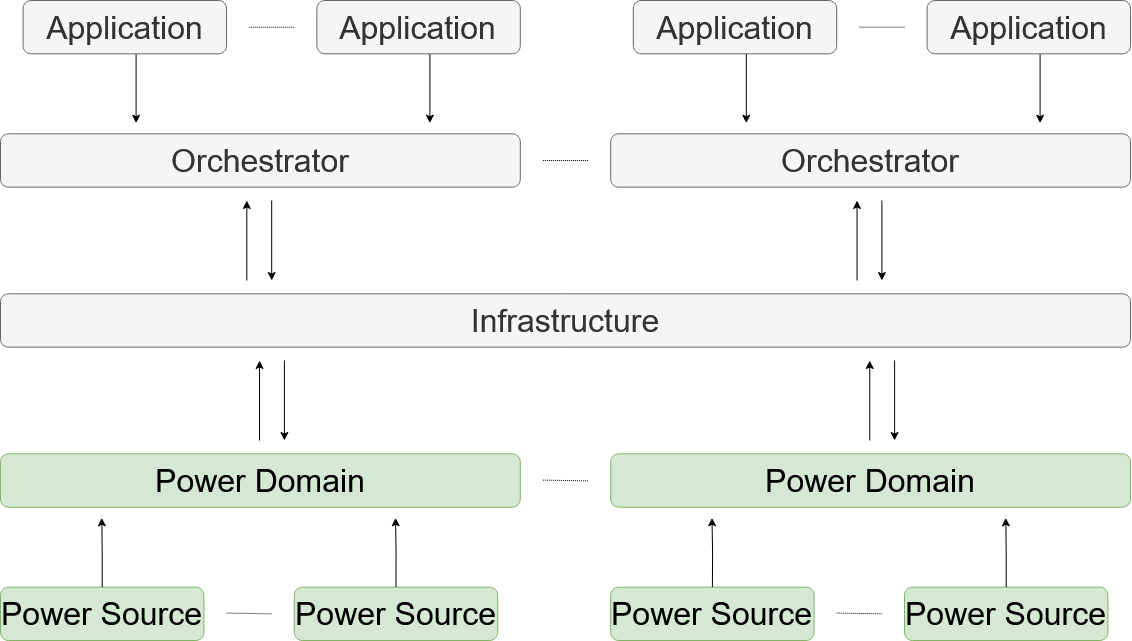
\includegraphics[width=0.9\textwidth]{images/Architecture.pdf}
    ~
    \caption{Architecture overview showing interactions between layers.}
    \label{fig:archtecture}
\end{figure}

As we can see, similar to how the orchestrator class mediates the relationships between the application and infrastructure layer, Extended LEAF allows interactions to occur between the power source and infrastructure layer through power domains.

\section{Fundamentals of Extended LEAF}
The following subsections go onto discuss the fundamental concepts used in developing Extended LEAF, these cover the ideas and techniques that are common throughout the framework and act as to how the simulation can take place.

\subsection{Discrete Event Simulations}\label{imp:subsec:des}
As briefly mentioned in Section \ref{subsec:power-domain-workflow} LEAF and subsequently Extended LEAF forward time through DESs.
Extended LEAF incorporates this through the use of the Python SimPy package \cite{simpy}.
Looking at Listing \ref{lst:simpy} we can provide an example to show how the SimPy package can create a simulation instance and execute code periodically:
\begin{lstlisting}[language=python, numbers=left, caption={Example use of the SimPy environment}, label=lst:simpy]
    def driver_Method():
        env = simpy.Environment()
        env.process(task(env))
        env.run(until=10)  # Run simulation for 10 units of time

    def task(env):
        while True:
            current_time = env.now()
            print(f"Task has been ran at time increment {current_time}")
            yield env.timeout(2)

    driver_Method()  # Run driver method
\end{lstlisting}
\begin{lstlisting}[language=TeX, caption={Terminal output of Listing \ref{lst:simpy}}, label=lst:simpy-output]
Task has been run at time increment 0
Task has been run at time increment 2
Task has been run at time increment 4
Task has been run at time increment 6
Task has been run at time increment 8
\end{lstlisting}

In this, we can see that the Environment() class is used to declare and initialise the simulation, keeping a reference to the env variable.
The example then informs the model to execute the task method inside the simulation environment by invoking process() with the task method call passed as a parameter.
Finally, the simulation's terminating condition is defined by passing an explicit value for the until argument, signalling that the simulation will terminate when the simulation's internal clock equals 10.
To allow the task method to be considered an `event' by the SimPy environment, it must be considered a ``Python generator'', where the yield environment.timeout() is inside the body of the method to allow the state of the model to progress forward in time.
In order to allow for the task to be called periodically, the task method encloses the logic of its body inside an indefinite while loop and uses yield environment.timeout(2) to pause the simulation for two units of time.
Fundamentally, Extended LEAF uses this approach to allow the power domain to execute its workflow on the model's most current state during the simulation.

\subsection{Time}\label{imp:subsec:time}
Now that we have explained how Extended LEAF uses SimPy to facilitate DESs and can progress the model forward in time, we can discuss how and why the implementation does this.
As a consequence of the implementation using historical data that is associated with an exact 24-hour time, \textit{the topic discussed in the upcoming section}, Extended LEAF needs the means to go from an integer-based representation of time to one that is formatted as HH\%MM\%SS.
This is achieved by having the simulation assume that for every increment of 1 in the simulation's internal clock, a minute or 60 seconds passes inside the environment space.
A minute was chosen because the simulation could avoid taking unnecessary measurements of the simulation for small periods where the model's state is unlikely to change but still capable of capturing changes in the state that would only occur in a relatively short period.
However, in simulations that execute for periods longer than 24 hours (1440 seconds), it is still necessary to allow the simulation to identify the current state uniquely, something that cannot occur when time is represented as HH\%MM\%SS. Therefore, Extended LEAF identifies the current state of a simulation at any given moment by using the clock's internal representation through env.now(), as any changes in the current state cause the time to progress within the simulation space.
This ensures that when data is written to a file, entries logged by the power domain will not get overwritten as they both uniquely represent the same time.

\subsection{Accessing Data}\label{imp:subsec:daa}
A core requirement of the project was to allow for fluctuations in power availability. Extended LEAF models a power source's power availability and carbon intensity as values that are updated every step forward in time.
When the simulation moves forward in time, a power source will determine its available power and carbon intensity that it should have at that corresponding moment.
For cases where power availability fluctuates (power sources that are not assumed to have a constant rate of power generation), the power source will consult a dictionary of corresponding (time, power) pairings using the current time of the simulation to produce the key to determine its power.
This data is loaded from a formatted CSV file when the class is initialised and provides data for 24 hours, where mechanisms within Extended LEAF return to the start when the end has been reached.
Because the original datasets differed in the rate at which measurements of power throughput were captured, there are discrepancies in time granularity for when a power source sees a change in available power.
For instance, one data set that fluctuates aggressively may have a reading every minute to capture this property.
In contrast, a power source with reasonably minimal changes in power may only have readings every 30 minutes.
To resolve this, Extended LEAF assumes that between changes in power readings, the power source maintains the previous rate until a new value can be retrieved.
This can be seen in Listing \ref{lst:time} which demonstrates how this assumption is implemented.\\

\begin{lstlisting}[language=python, numbers=left, caption={Example use of how a power source accesses it's available power.}, label=lst:time]
    def get_power_at_time(self, time_int) -> float:
        time = self._map_to_time((time_int // self.update_interval) % len(self.power_data))
        return float(self.power_data[time])
\end{lstlisting}

In order to find the appropriate key to determine the power available, the method carries out a floor division between the current time and the difference in time between readings to find the most recent time.
The implemented mechanism that allows simulations to occur for periods longer than 24 hours operates by wrapping the current time key back to the start of the data.
This is done by applying the modulus of the dictionary's size to this value.
From this, \_map\_to\_time() is used to convert this integer representation of time to a 24-hour string key to obtain the correct power from the dictionary.
To help illustrate this idea, Table \ref{tab:data-dic} visualises the first ten minutes of a potential example dictionary.
Table \ref{tab:time-explanation} describes how this data describes the first 10 minutes of this power source's availability.
\begin{table}[h]
    \rowcolors{2}{}{gray!3}
    \caption{Table depicting the data held in file}
    \label{tab:data-dic}
    \centering
    \begin{tabular}{@{}ccc@{}}
    \toprule
    \textbf{Time} & \textbf{Power} \\
    \midrule
    12:00:00      & 102            \\
    12:05:00      & 114            \\
    12:10:00      & 127            \\
    \bottomrule
    \end{tabular}

    \vspace{1em} % Add some vertical space between the tables
    \rowcolors{2}{}{gray!3}
    \caption{Table depicting how in reality power would be read from a power source's dictionary}
    \label{tab:time-explanation}
    %\tt
    \begin{tabular}{@{}lll@{}}
    \toprule
    \textbf{Env.now()}    & \textbf{Key}       & \textbf{Power}     \\
    \midrule
    0                     & 12:00:00           & 102                \\
    1                     & 12:00:00           & 102                \\
    2                     & 12:00:00           & 102                \\
    3                     & 12:00:00           & 102                \\
    4                     & 12:00:00           & 102                \\
    5                     & 12:05:00           & 114                \\
    6                     & 12:05:00           & 114                \\
    7                     & 12:05:00           & 114                \\
    8                     & 12:05:00           & 114                \\
    9                     & 12:05:00           & 114                \\
    10                    & 12:10:00           & 127                \\
    \bottomrule
    \end{tabular}
\end{table}

\section{Providing Power and Calculating Carbon Emissions}

\subsection{The Power Domain}\label{sec:power-domain}
The power domain is implemented in Extended LEAF through the class type of PowerDomain.
To introduce the power domain within the simulation space, the user must initialise an instance of the class and pass an instance of its run method into the environment.
When initialising an instance, the user configures the power domain by passing through these items:
\begin{itemize}
    \item \textbf{env}, this is the reference to the Environment() class used to simulate the model.
    \item \textbf{name}, the name of the power domain. This value must be unique as it identifies the power domain.
    \item \textit{(Optional)} \textbf{start\_time\_str}, this is the string time for when the simulation should start. \textbf{powered\_infrastructure}, these are the entities the user wants to immediately assign to a power source dynamically.
    \item \textit{(Optional)} \textbf{powered\_infrastructure\_distributor}, the custom entity distribution method. NB, this replaces the default implementation provided by Extended LEAF.
\item \end{itemize}

\subsubsection{Utility Functions}\label{imp:subsec:utility}
As the power domain is the focus of the features provided in Extended LEAF, the class provides an array of methods that allow the workflow to carry out its tasks.

When a power domain is initialised, it may have been apparent that no power sources are passed through the constructor argument;
this is because the first feature provided by the power domain is add\_power\_source(), which creates these associations between a power source and a power domain().
When the power domain invokes add\_power\_source(), the power source's priority is used to insert the power domain into the correct location within the power domain's list data structure power\_sources.
When a power domain no longer wishes to associate with a power source, it invokes the instance method remove\_power\_source ().
This is to ensure that the power source is correctly removed from the power domain and that any entities currently powered by it are safely removed.
Adding and removing power sources allows users to describe scenarios where a power source may become available or unavailable during the simulation;
this could potentially model external factors such as power cuts.

The power domain's following core utility function is the ability to create and remove associations between infrastructure entities and the power domain.
The power domain achieves this by calling add\_entity() and remove\_entity(), respectively.
Similar to those for the power sources, add\_entity() and remove\_entity() safely add and remove infrastructure entities to the power domains list structure powered\_infrastructure.
This feature could be useful by considering the proposed events system, where the dynamic mobility of entities within the network allows them to move from one power domain to another. For instance, a mobile phone being charged at one site and then another.

The final core feature of the power domain is the function used to calculate the amount of carbon produced.
As a core goal of the project was to introduce this ability, it was critical to provide this feature somewhere accessible to most classes.
Listing \ref{lst:calc-carbon} shows that the class function takes as arguments the energy consumed (in watt-hours) and a power source's current carbon intensity to calculate the amount of carbon released.
\begin{lstlisting}[language=python, numbers=left, caption={Listing showing the class method used to calculate carbon emissions.}, label=lst:calc-carbon]
    @classmethod
    def calculate_carbon_released(cls, power_used, carbon_intensity) -> float:
        return float(power_used) * (10 ** -3) * float(carbon_intensity)
\end{lstlisting}

Finally, the power domain also provides various small class functions to carry out common tasks, for instance convert\_to\_time\_string() and get\_current\_time().

\subsubsection{Workflow}\label{imp:subsec:workflow}
As discussed in Section \ref{subsec:power-domain-workflow}, the workflow of the power domain is where the main interactions between the Power and Infrastructure layers occur.
Extended LEAF implements this workflow by providing an invokable run method for an instance of the PowerDomain class.
Using the ideas presented in Section \ref{imp:subsec:des}, this method is passed through into the simulation environment to progress the simulation forward in time.

The power domain combines tasks in the workflow into the same body of a for loop when possible to minimise iterating through the power sources multiple times.
In addition, the power domain takes advantage of the ordering of its power\_sources list. It uses this to iterate through each power source, as the source's priority determined the position within this list when the power source was added.

The first for loop iterates through power\_sources in order to define each power source's available power and carbon intensity at that moment in the simulation.
This is necessary before the next for loop, as the distribution process in the following stage considers the power and carbon intensity of other power sources. Therefore, these must be updated before the following stages occur.

Once all the power sources have their values updated, each power source determines the infrastructure entities it will power for the current time step and logs its measurements.
We can take measurements at this stage because Extended LEAF iterates through power sources in the order of most desirable as explained in \ref{subsec:distributing-entities}.
Because of this, once a dynamic power source receives its allocated entities from the power domain, these entities will remain there until time moves forward.
For static power sources, rather than receive entities through the distribution method, evaluate those with a constant relationship.

Finally, the workflow evaluates whether all entities possess an association with a power source; if this is not true, the simulation fails by raising an error.
\subsubsection{Distributing Entities to Power Sources}\label{imp:subsec:distributor}
The power domain uses the PoweredInfrastructureDistributor class to distribute entities within the infrastructure to power sources.
The class contains only two attributes:
\begin{itemize}
    \item \textbf{powered\_infrastructure\_distributor\_method}, this is the method which determines entities for a given power source.
    \item \textbf{smart\_distribution}, this is used within the default method to allow for advanced features.
\end{itemize}
The class is initialised in one of two ways: letting the framework initialise a default implementation or creating a custom instance with a custom distribution method.

For context, when a power source evaluates an entity, an inequality comparison is carried out between the power source's available power and an entity's power requirements.
When the power domain calls the distributor method, it passes in two items: the power source which wants to receive entities and the power domain itself.
The method receives the power domain in order to see the entities within it.
The method then selects and returns the most appropriate entities for a given power source.

As defined in Section \ref{subsec:distributing-entities}, the entities are separated into three categories.
The first category evaluated is the entities that the power source powered in the previous state of the simulation.
It evaluates these first as the system assumes that these should try to retain an association before distributing power elsewhere.
If the source can no longer power one of these entities, the entity the power source removes it from its list of powered\_infrastructure.

After this, the method evaluates entities that have no power source.
It evaluates these entities second, as the simulation would fail if an entity could not be assigned a power source.
If an entity here can join the power source, the method adds the entity to the power source's powered\_infrastructure.

Finally, the method uses the instance's smart\_distribution attribute and the current power source's priority to try to power entities from less desirable power sources.
This process occurs last because the categories above take more precedence over this one.
If an entity can join the power source, it is first removed from the previous power source's list of powered\_infrastructure and added to its own.

\subsubsection{Logging Results}\label{imp:subsec:logging-results}
The power domain implements the ability to record measurements about the simulation's current state by building a nested dictionary as it moves forward in time.
The benefit of working with nested dictionaries is that this can be easily transformed into a JSON file to write a file later on, and amendments can be made when appropriate.
Appendix \ref{lst:dic-log} shows an example of this tree-like structure.
The results of the simulation are structured hierarchically.
The outer dictionary contains information about the entire simulation.
The next level describes the state of the environment at any given moment.
The layer after this defines the current state of each power source.
Finally, the innermost state describes the measurements of the entities.
By organising items in the simulation this way, the power domain eliminates the need to explicitly describe associations, reducing redundancy and the size of results.
The listing shows that the dictionary's power source level also describes particular attributes of the power source.
This is done to keep a record of the power source at that moment during the simulation's runtime.
These values can later be used when analysing results.

\subsection{Power Sources}\label{sec:power-sources}
Power sources are implemented in Extended LEAF using an abstract class to define the class instances' universal attributes and methods.
By using abstract classes, the user can focus on defining the logic unique to a particular power source without having to consider implementing the functionality already defined in the abstract class.
Because the power domain only considers a few abstract methods, the effort required to develop custom implementations of power sources is minimal.
As discussed in Section \ref{sec:power-sources}, power sources are classified through two distinct features: their type and whether they are a static or dynamic power source.
The power type of a power source is implemented through an enumerator to describe the three potential types that exist: RENEWABLE, MIXED and BATTERY.
If the user wishes for a power source to maintain a constant relationship with a collection of entities, then the static argument must be set to True in the constructor along with providing the entities they wish to have an association.\\
Extended LEAF initialises power sources by defining a concrete instance of the PowerSource class.
These instances are designed to simulate the characteristics of the power sources they are based on.

While the user can develop their own power sources, Extended LEAF provides four main examples: Solar Power, Wind Power, Grid Power, and Battery Power.
These power sources take from real-life historical data to define their behaviour in each state of the simulation.
For instance, renewable power sources (SolarPower and WindPower) retrieve data for their power availability (with the default data being provided from EirGrid \citep{eirgrid}), whereas non-renewable power sources (GridPower) retrieve data for their carbon intensity (with the default data being provided from the Carbon Intensity API \citep{carbon_intensity_api}).
Finally, the BatteryPower class is unique, as it stores power rather than generates it.
This source acts differently and only updates naturally to return to full power once another power source charges it.
Suppose the user wishes to implement their own power source.
In that case, they are expected to define the logic for updating and providing information about the current power available and the carbon intensity at that moment in time.

Power sources provide the user the ability to configure them in a variety of ways.
The user achieves this through the arguments they provide during the initialisation of the instance:
\begin{itemize}
    \item \textbf{env}, the reference to the Environment() class used to simulate the model.
    \item \textbf{name}, the name of the power source, like the power domain, must be kept unique as it is used to identify itself.
    \item \textbf{data\_set\_filename}, this is the file path for the data that fluctuates: either the carbon intensity or available power.
    \item \textbf{power\_domain}, this is power domain instance. NB, this is required to acknowledge the time the simulation starts.
    \item \textbf{priority} is the integer that describes preference when distributing entities where 0 is the most important.
    \item \textit{(Optional)} \textbf{static}, this is a boolean flag to signal to the power domain, not to distribute entities to this power source.
    \item \textit{(Optional)} \textbf{powered\_infrastructure}, these are the entities the user wants to assign to a power source statically.
\end{itemize}
The PowerSource class represents the available power at any given moment in time by using a floating point variable \textit{remaining\_power}.
While \cite{leaf2021} uses a power model in the Application and Infrastructure layer to represent static and dynamic power consumption, Extended LEAF only needs a single value.
To convert from a PowerModel reading of power to a single value, the power domain casts the type as a float to retrieve the required power.

\subsubsection{Evaluating Entities within Static Power sources}\label{imp:subsec:static-entities}
While the PoweredInfrastructureDistributor class distributes entities to dynamic power sources, static power sources also need to determine what entities they will power at each moment in the simulation.
Because of this, the power source provides a crucial method called \textbf{evaluate\_entities}.
The purpose of this method, \textit{just like the powered\_infrastructure\_distributor\_method}, is to determine which entities are powered at the current state of the simulation for static power sources.
It achieves this by iterating through each entity present and carrying out the same evaluation discussed in Section \ref{imp:subsec:distributor}.
However, as the power source is considered static, the method cannot simply free the entity back to the power domain for another power source to power.
Instead, the power source effectively turns off the entity by pausing it and removing any tasks or dataflows in the entity itself and the remaining application.

\subsubsection{Functionality}\label{imp:subsec:utility-funcs}
Like the PowerDomain class, the abstract class of PowerSource provides the user with a range of functions available to all realised instances of the class.
Unlike the abstract methods, which are specialised to each individual concrete class of PowerSource, these methods provide the same functionality throughout all instances.

The first collection of functions the PowerSource class provides is related to power consumption.
These include providing safe approaches in consuming (\textit{consume\_power()}), setting (\textit{set\_current\_power()}) and retrieving power (\textit{get\_current\_power()}).
Because of this, when the simulation needs to interact with the current remaining power of a power source, they can call these methods without worrying about providing checks to ensure correctness.
The PowerSource class also provides essential add and remove methods to include and drop entities from within their list of powered\_infrastructure.
Similar to the PowerDomain class, these add and remove methods correctly ensure that when an entity is handled by the power source, the necessary processes have occurred to prevent entities from not being correctly updated.

Finally, the PowerSource class is also responsible for processing the data regarding the particular power source instance.
In addition, the method processes the data to start at the user's desired time, allowing users to define when a simulation can start without having to move the simulation's internal clock forward to achieve this.

\section{Events}\label{imp:sec:envts}
Extended LEAF implements events in the framework by introducing Event and EventDomain classes.
Similar to the definition used to describe events in DESs \citep{Des}, an Event instance in this context describes a method that will be executed at some point during the simulation.
An instance of EventDomain manages these events and moves independently within the simulation, executing them when appropriate.

\subsection{Events}\label{imp:subsec:event-class}
The Event class aims to inform an instance of EventDomain how and when to execute a callback method.
Because of this, the class provides no functionality besides being initialised.
An event is described through the following attributes:
\begin{itemize}
    \item \textbf{event}, this is the method the user wants to execute. NB, the user should only reference the method; therefore, no parentheses are included.
    \item \textbf{args}, this is a list of the arguments that must be passed into the method.
    \item \textbf{time\_str}, this is the (string) time when the event should execute. NB, this should be formatted as HH\%MM\%SS.
    \item \textit{(Optional)} \textbf{repeat}, this is a boolean flag to signal whether the event should execute after a certain amount of time has elapsed.
    \item \textit{(Optional)} \textbf{repeat\_counter}, following from repeat, this indicates how much time should elapse in minutes before the event executes again.
\end{itemize}

\subsection{Managing Events}\label{imp:subsec:event-domain-class}
As previously mentioned, the goal of the EventDomain class is to manage when events are executed within the simulation.
Just like the Event class, the EventDomain instance is expected to be initialised by the user by considering the environment (env), the amount of time elapsed between considering events (update\_interval) and the time the manager starts running (start\_time\_str).

When the user defines the simulation model, instances of the Events class are associated with the event domain by calling the add\_event() method.
Like the PowerDomain class, the EventDomain moves independently within the simulation space using the same approach outlined within Section \ref{imp:subsec:time}, where a driver method is used to iterate constantly through time within the simulation.
When the event domain does move forward in time, the driver method calls the only other method available run\_events().

The run\_events() method operates by first finding the current time of the simulation and initialising an empty list.
The purpose of this list is to identify any events that have been executed during this time interval of the simulation so they can be safely removed afterwards.
The method then proceeds to iterate through its events.
During this, each event is evaluated using an inequality comparison.
If the current time equals or surpasses an event's execution time, the event's method is called passing in any provided arguments.
If the user wishes for an event to be repeated and executed regularly, a new event instance is created by copying over the attributes of the old event, with the execution time incremented.
After this, the event is added to the event\_history list data structure to log executed events.
Finally, the old event is flagged and ready to be deleted once all other events have been run.

\section{Results}\label{sec:displaying-results}
TThe final aspect introduced into Extended LEAF is the ability to store and display results.
Using the data logged from Section \ref{imp:subsec:logging-results} Extended LEAF allows the data generated during the simulation to be saved to a file and visualised through graphs and animations.
It achieves this by using the Python packages Plotly \citep{plotly-git}, Matplotlib \citep{Hunter:2007} and NetworkX \citep{networkx}.
Once the simulation has finished executing, the user is free to analyse the data however they deem fit.
Extended LEAF provides the user with three classes to view the data:

\begin{enumerate}
    \item FileHandler
    \item FigurePlotter
    \item Animation
\end{enumerate}

\subsection{File Handling}\label{subsec:imp:filehandler}
The FileHandler class saves writable objects to a file.
Similar to the native FileHandler class in Python \citep{python-docs-FileHandler}, the FileHandler class in Extended LEAF provides the necessary features to write both the power domain's results of the simulation and any graphs generated to the file.
It achieves this by creating a unique directory within the results folder. The folder's name reflects the file from which the FileHandler was initialised, along with a date and time stamp.
If the user wants to use the class, they are expected to initialise an instance.
This class was implemented to keep the user's focus of Extended LEAF on creating simulations rather than dealing with file writers.

\subsection{Plotting Graphs}\label{subsec:imp:figureplotter}
The user can generate automated graphs of the simulation by utilising the FigurePlotter class.
This class's goal is to provide a collection of functions that can be used to generate instances of Plotly.Figure.
If the user wants to use this class, then an instance of it must be initialised by passing through the following items:
\begin{itemize}
    \item \textbf{power\_domain}, the power domain from which the user wants to produce results.
    \item \textit{(Optional)} \textbf{event\_domain}, the event domain that issued any events in the same simulation space as power\_domain.
    \item \textit{(Optional)} \textbf{show\_event\_lines}, this is a boolean flag for a stylistic choice to have lines that intersect events cut through other figures.
    \item \textit{(Optional)} \textbf{(number\_of\_divisions)}, this is an integer used to indicate how many x-ticks there should be.
    \item \textit{(Optional)} \textbf{title}, this is the overall title if an aggregated figure is used.
\end{itemize}
Once an instance has been defined, the user can invoke the instance and generate a figure by calling any of these methods:
\begin{itemize}
    \item subplot\_time\_series\_entities()
    \item subplot\_time\_series\_power\_sources()
    \item subplot\_time\_series\_power\_meter()
\end{itemize}
By passing through the desired attribute and necessary instances to plot, the methods return an instance of Plotly.Figure.\\
Finally, the class can reduce the number of figures present by aggregating the graphs into the same figure and converting the existing figure into sub-figures.
Figure \ref{fig:dev-example7-results} shows an example of the graphs that can be generated from this class.
\begin{figure}[h]
    \centering
    \includegraphics[width=\textwidth]{images/dev_examaple7_results.pdf}
    ~
    \caption{Example figure generated from 7\_extended\_file\_writer.py in the development\_examples folder.}
    \label{fig:dev-example7-results}
\end{figure}

\subsection{Animating Results}\label{subsec:imp:animation}
The last major class Extended LEAF saw to provide was a means to visualise how infrastructure entities interacted with power sources during the simulation.
This class was needed during development to evaluate the examples produced alongside the framework, as having textual descriptions of relations in the debugger used did not provide enough detail about how entities were being distributed among power sources.

The Animation class achieves this by providing an interactive means to move through each simulation state and view the relations between entities and power sources.
It implements this using the Matplotlib and NetworkX packages to place a series of graphs over an interactive plot.
When the play button is pressed or the slider moves across the time series, a new NetworkX graph is generated.
When this happens, an index of that current moment is used to generate the relationships that existed by inspecting the corresponding entry in the power domains log using the key values to decide.
Figure \ref{fig:dev-example7-animation} shows an example instance of this animation.
\begin{figure}[h]
    \centering
    \includegraphics[width=\textwidth]{images/example7-animation.pdf}
    ~
    \caption{Example figure generated from 7\_extended\_file\_writer.py in the development\_examples folder.}
    \label{fig:dev-example7-animation}
\end{figure}

%==================================================================================================================================

\chapter{Evaluation} \label{chp:evaluation}
%How good is your solution? How well did you solve the general problem, and what evidence do you have to support that?

To Evaluate Extended LEAF various scenarios under a single context have been developed to demonstrate the framework's functionality.
The intention behind these scenarios is to provide evidence that the framework correctly introduces the classes discussed in Chapter \ref{chp:imp}.
As the section progresses, the scenarios will become detailed and increase in complexity until arriving at the final example demonstrating a complete scenario.

\section{Experimental Setup}\label{eval:sec:scenarios}

% E. E. Agency, “CO2 emission intensity,” 2020. [Online]. Available: https:
%//www.eea.europa.eu/data-and-maps/daviz/co2-emission-intensity-9
for carbon intensities

\subsection{Context Background}\label{eval:subsec:precision-agriculture}
- describe precision agriculture
- why it is a great scenario to use
- reference where the data was retrieved from

\section{Scenarios 1 - A Singular Static Power Source}\label{eval:subsec:scenario1}
Scenario 1 provides the simplest use case of Extended LEAF and describes a static grid power source with 3 nodes.
For context, the scenario explores a 9 minute event where soil moisture readings are being captured in real time and pre-processed before being transmitted to a remote server.
The goal of this scenario is to demonstrate that entities within the infrastructure are allocated power and  produce carbon emissions as a result of being associated to a power source.
As we can see, Figure \ref{fig:example1_diagram} demonstrates how the power, infrastructure and application layers interact.

\begin{figure}[h]
    \centering
    \includegraphics[width=0.4\textwidth]{images/examples/example_1/example1_diagram.pdf}
    ~
    \caption{Illustration depicting scenario 1.}
    \label{fig:example1_diagram}
\end{figure}

\textit{For results please refer to Appendix \ref{apen:subsec:scen1}}.\\

\subsection{Scenario 1 Analysis}
Looking at the results we can see that despite the basic nature of the scenario, Figures \ref{fig:example1-1} and \ref{fig:example1-2} indicate that the correct amount of power is being consumed from the power source.
This can be seen as when at any given moment in time, the entities in Figure \ref{fig:example1-1} when summed equal the corresponding point in Figure \ref{fig:example1-2}.
When inspecting the amount of carbon released the same behaviour can also be seen there too, as \ref{fig:example1-0} and \ref{fig:example1-3} show the same relationship between the carbon released for individual entities and the grid power source.
This makes sense as when examining the equation for carbon intensity as defined in Section \ref{subsec:carbon-released}, we can see that both power and carbon released are proportional to one another.

\section{Scenarios 2 - Multiple Dynamic Power Sources}\label{eval:subsec:scenario2}
\begin{figure}[h]
    \centering
    \includegraphics[width=0.9\textwidth]{images/examples/example_2/example2_diagram.pdf}
    ~
    \caption{Illustration depicting scenario 2.}
    \label{fig:example2_diagram}
\end{figure}

\section{Scenarios 3 - A Custom Infrastructure Distributor}\label{eval:subsec:scenario3}
\begin{figure}[h]
    \centering
    \includegraphics[width=0.9\textwidth]{images/examples/example_3/example3_diagram.pdf}
    ~
    \caption{Illustration depicting scenario 3.}
    \label{fig:example3_diagram}
\end{figure}

\section{Scenarios 4 - An Off-Peak Battery Power Source}\label{eval:subsec:scenario4}
\begin{figure}[h]
    \centering
    \includegraphics[width=0.9\textwidth]{images/examples/example_4/example4_diagram.pdf}
    ~
    \caption{Illustration depicting scenario 4.}
    \label{fig:example4_diagram}
\end{figure}

\section{Scenarios 5 - A Carbon Aware Application Orchestrator}\label{eval:subsec:scenario 5}
\begin{figure}[h]
    \centering
    \includegraphics[width=0.9\textwidth]{images/examples/example_5/example5_diagram.pdf}
    ~
    \caption{Illustration depicting scenario 5.}
    \label{fig:example5_diagram}
\end{figure}

\section{Scenarios 6 - Cyclic Infrastructure Pausing}\label{eval:subsec:scenario 6}
\begin{figure}[h]
    \centering
    \includegraphics[width=0.9\textwidth]{images/examples/example_6/example6_diagram.pdf}
    ~
    \caption{Illustration depicting scenario 6.}
    \label{fig:example6_diagram}
\end{figure}

\section{Scenarios 7 - Precision Agriculture}\label{eval:subsec:scenario 7}
\begin{figure}[h]
    \centering
    \includegraphics[width=0.9\textwidth]{images/examples/example_7/example7_diagram.pdf}
    ~
    \caption{Illustration depicting scenario 7.}
    \label{fig:example7_diagram}
\end{figure}
\begin{figure}[h]
    \centering
    \includegraphics[width=\textwidth]{images/examples/example_7/Main_results}
    ~
    \caption{Graphs depicting the timeseries of total carbon emissions for power sources}
    \label{fig:example7_final_results}
\end{figure}

%When the user sets out to carry out a simulation, the user should reference Figure \ref{fig:archtecture} and work from the bottom up
%\section{Running Simulations}\label{imp:sec:running-simulations}
%
%
%\section{Guidance}
%\begin{itemize}
%    \item
%        Ask specific questions that address the general problem.
%    \item
%        Answer them with precise evidence (graphs, numbers, statistical
%        analysis, qualitative analysis).
%    \item
%        Be fair and be scientific.
%    \item
%        The key thing is to show that you know how to evaluate your work, not
%        that your work is the most amazing product ever.
%\end{itemize}
%
%Make sure you present your evidence well. Use appropriate visualisations, reporting techniques and statistical analysis, as appropriate.

%%If you visualise, follow the basic rules, as illustrated in Figure \ref{fig:boxplot}:
%\item Label everything correctly (axis, title, units).
%\item Caption thoroughly.
%\item Reference in text.
%\item \textbf{Include appropriate display of uncertainty (e.g. error bars, Box plot)}
%\item Minimize clutter.


%==================================================================================================================================
\chapter{Conclusion}

\section{limitations}
- Assume grid power is unlimited
- assume that carbon released is a product of the infrastructure not the power source
- recharging the battery occurs instantaneously

\section{Future Work}\label{conc:sec:Future Work}
\section{Personal Reflection}\label{conc:sec:Personal Reflection}

%Summarise the whole project for a lazy reader who didn't read the rest (e.g. a prize-awarding committee).
%\section{Guidance}
%\begin{itemize}
%    \item
%        Summarise briefly and fairly.
%    \item
%        You should be addressing the general problem you introduced in the
%        Introduction.
%    \item
%        Include summary of concrete results (``the new compiler ran 2x
%        faster'')
%    \item
%        Indicate what future work could be done, but remember: \textbf{you
%        won't get credit for things you haven't done}.
%\end{itemize}
%- mention future intrest and collaborations with other students
%- mention to incorperate an automatic priorising system to allow for dynamic carbon intensity sources like Grid to have their priority change
%- mention that possiblity to introduce priority of nodes/tasks (either or) as currently the model does not preference particular tasks when determining where/ when they are associated to a power source
%==================================================================================================================================
%
% 
%==================================================================================================================================
%  APPENDICES  
\begin{appendices}
\chapter{Appendices}

\section{Dictionary log Example}
\begin{lstlisting}[caption={Example dictionary structure used by the power domain.},label={lst:dic-log}]
{
    "0": {
        "Wind Power Source": {
          "Node A": {
            "Power Used": 0.1,
            "Carbon Intensity": 1,
            "Carbon Released": 0.1
          },
          "Total Carbon Released": 0.1,
          "Power Available": 99.9
        },
        "Solar Power Source": {
          "Node B": {
            "Power Used": 0.06,
            "Carbon Intensity": 2,
            "Carbon Released": 0.12
          },
          "Node C": {
            "Power Used": 0.15,
            "Carbon Intensity": 1,
            "Carbon Released": 0.15
          },
          "Total Carbon Released": 0.27,
          "Power Available": 19.78
        }
    },
    "1": {
        "Wind Power Source": {
          "Node A": {
            "Power Used": 0.15,
            "Carbon Intensity": 2,
            "Carbon Released": 0.30
          },
          "Node B": {
            "Power Used": 0.03,
            "Carbon Intensity": 2,
            "Carbon Released": 0.06
          },
          "Total Carbon Released": 0.36,
          "Power Available": 99.82
        },
        "Solar Power Source": {
          "Node C": {
            "Power Used": 0.15,
            "Carbon Intensity": 1,
            "Carbon Released": 0.15
          },
          "Total Carbon Released": 0.27,
          "Power Available": 19.85
        }
    }
}
\end{lstlisting}
Typical inclusions in the appendices are:

\begin{itemize}
\item
  Copies of ethics approvals (required if obtained)
\item
  Copies of questionnaires etc. used to gather data from subjects.
\item
  Extensive tables or figures that are too bulky to fit in the main body of
  the report, particularly ones that are repetitive and summarised in the body.

\item Outline of the source code (e.g. directory structure), or other architecture documentation like class diagrams.

\item User manuals, and any guides to starting/running the software.

\end{itemize}

\textbf{Don't include your source code in the appendices}. It will be
submitted separately.

\clearpage
\section{Scenario 1 Results}\label{apen:subsec:scen1}
The Following appendices are the results for scenario 1.
\clearpage
\begin{figure}[htbp]
    \centering
    \includegraphics[width=1.5\textwidth,angle=270]{images/examples/example_1/example_1-0}
    ~
    \caption{Graph showing the timeseries of carbon released for powered infrastructure.}
    \label{fig:example1-0}
\end{figure}
\clearpage
\begin{figure}[htbp]
    \centering
    \includegraphics[width=1.5\textwidth,angle=270]{images/examples/example_1/example_1-1}
    ~
    \caption{Graph showing the timeseries of energy consumed for powered infrastructure.}
    \label{fig:example1-1}
\end{figure}
\clearpage
\begin{figure}[htbp]
    \centering
    \includegraphics[width=1.5\textwidth,angle=270]{images/examples/example_1/example_1-2}
    ~
    \caption{Graph showing the timeseries of energy consumed for power sources.}
    \label{fig:example1-2}
\end{figure}
\clearpage
\begin{figure}[htbp]
    \centering
    \includegraphics[width=1.5\textwidth,angle=270]{images/examples/example_1/example_1-3}
    ~
    \caption{Graph showing the timeseries of carbon released for power sources.}
    \label{fig:example1-3}
\end{figure}

\clearpage
\section{Scenario 2 Results}\label{apen:subsec:scen2}
The Following appendices are the results for scenario 2.
\begin{figure}[htbp]
    \centering
    \includegraphics[width=1.5\textwidth,angle=270]{images/examples/example_2/example_2-0}
    ~
    \caption{Graph showing the timeseries of carbon released for powered infrastructure.}
    \label{fig:example2-0}
\end{figure}
\clearpage
\begin{figure}[htbp]
    \centering
    \includegraphics[width=1.5\textwidth,angle=270]{images/examples/example_2/example_2-1}
    ~
    \caption{Graph showing the timeseries of energy consumed for powered infrastructure.}
    \label{fig:example2-1}
\end{figure}
\clearpage
\begin{figure}[htbp]
    \centering
    \includegraphics[width=1.5\textwidth,angle=270]{images/examples/example_2/example_2-2}
    ~
    \caption{Graph showing the timeseries of energy consumed for power sources.}
    \label{fig:example2-2}
\end{figure}
\clearpage
\begin{figure}[htbp]
    \centering
    \includegraphics[width=1.5\textwidth,angle=270]{images/examples/example_2/example_2-3}
    ~
    \caption{Graph showing the timeseries of carbon released for power sources.}
    \label{fig:example2-3}
\end{figure}
\clearpage
\section{Scenario 3 Results}\label{apen:subsec:scen3}
The Following appendices are the results for scenario 3.
\clearpage
\begin{figure}[htbp]
    \centering
    \includegraphics[width=1.5\textwidth,angle=270]{images/examples/example_3/example_3-0}
    ~
    \caption{Graph showing the timeseries of carbon released for powered infrastructure.}
    \label{fig:example3-0}
\end{figure}
\clearpage
\begin{figure}[htbp]
    \centering
    \includegraphics[width=1.5\textwidth,angle=270]{images/examples/example_3/example_3-1}
    ~
    \caption{Graph showing the timeseries of energy consumed for powered infrastructure.}
    \label{fig:example3-1}
\end{figure}
\clearpage
\begin{figure}[htbp]
    \centering
    \includegraphics[width=1.5\textwidth,angle=270]{images/examples/example_3/example_3-2}
    ~
    \caption{Graph showing the timeseries of energy consumed for power sources.}
    \label{fig:example3-2}
\end{figure}
\clearpage
\begin{figure}[htbp]
    \centering
    \includegraphics[width=1.5\textwidth,angle=270]{images/examples/example_3/example_3-3}
    ~
    \caption{Graph showing the timeseries of carbon released for power sources.}
    \label{fig:example3-3}
\end{figure}

\clearpage
\section{Scenario 4 Results}\label{apen:subsec:scen4}
The Following appendices are the results for scenario 4.
\clearpage
\begin{figure}[htbp]
    \centering
    \includegraphics[width=1.5\textwidth,angle=270]{images/examples/example_4/example_4-0}
    ~
    \caption{Graph showing the timeseries of events.}
    \label{fig:example4-0}
\end{figure}
\clearpage
\begin{figure}[htbp]
    \centering
    \includegraphics[width=1.5\textwidth,angle=270]{images/examples/example_4/example_4-1}
    ~
    \caption{Graph showing the timeseries of carbon released for powered infrastructure.}
    \label{fig:example4-1}
\end{figure}
\clearpage
\begin{figure}[htbp]
    \centering
    \includegraphics[width=1.5\textwidth,angle=270]{images/examples/example_4/example_4-2}
    ~
    \caption{Graph showing the timeseries of energy consumed for powered infrastructure.}
    \label{fig:example4-2}
\end{figure}
\clearpage
\begin{figure}[htbp]
    \centering
    \includegraphics[width=1.5\textwidth,angle=270]{images/examples/example_4/example_4-3}
    ~
    \caption{Graph showing the timeseries of energy consumed for power sources.}
    \label{fig:example4-3}
\end{figure}
\clearpage
\begin{figure}[htbp]
    \centering
    \includegraphics[width=1.5\textwidth,angle=270]{images/examples/example_4/example_4-4}
    ~
    \caption{Graph showing the timeseries of carbon released for power sources.}
    \label{fig:example4-4}
\end{figure}
\clearpage
\begin{figure}[htbp]
    \centering
    \includegraphics[width=1.5\textwidth,angle=270]{images/examples/example_4/example_4-5}
    ~
    \caption{Graph showing the timeseries of power used for power meters.}
    \label{fig:example4-5}
\end{figure}

\clearpage
\section{Scenario 5 Results}\label{apen:subsec:scen5}
The Following appendices are the results for scenario 5.
\clearpage
\begin{figure}[htbp]
    \centering
    \includegraphics[width=1.5\textwidth,angle=270]{images/examples/example_5/example_5-0}
    ~
    \caption{Graph showing the timeseries of events.}
    \label{fig:example5-0}
\end{figure}
\clearpage
\begin{figure}[htbp]
    \centering
    \includegraphics[width=1.5\textwidth,angle=270]{images/examples/example_5/example_5-1}
    ~
    \caption{Graph showing the timeseries of carbon released for powered infrastructure.}
    \label{fig:example5-1}
\end{figure}
\clearpage
\begin{figure}[htbp]
    \centering
    \includegraphics[width=1.5\textwidth,angle=270]{images/examples/example_5/example_5-2}
    ~
    \caption{Graph showing the timeseries of energy consumed for powered infrastructure.}
    \label{fig:example5-2}
\end{figure}
\clearpage
\begin{figure}[htbp]
    \centering
    \includegraphics[width=1.5\textwidth,angle=270]{images/examples/example_5/example_5-3}
    ~
    \caption{Graph showing the timeseries of energy consumed for power sources.}
    \label{fig:example5-3}
\end{figure}
\clearpage
\begin{figure}[htbp]
    \centering
    \includegraphics[width=1.5\textwidth,angle=270]{images/examples/example_5/example_5-4}
    ~
    \caption{Graph showing the timeseries of carbon released for power sources.}
    \label{fig:example5-4}
\end{figure}
\clearpage
\begin{figure}[htbp]
    \centering
    \includegraphics[width=1.5\textwidth,angle=270]{images/examples/example_5/example_5-5}
    ~
    \caption{Graph showing the timeseries of energy consumed for power sources.}
    \label{fig:example5-5}
\end{figure}

\clearpage
\section{Scenario 6 Results}\label{apen:subsec:scen6}
The Following appendices are the results for scenario 6.
\clearpage
\begin{figure}[htbp]
    \centering
    \includegraphics[width=1.5\textwidth,angle=270]{images/examples/example_6/example_6-0}
    ~
    \caption{Graph showing the timeseries of events.}
    \label{fig:example6-0}
\end{figure}
\clearpage
\begin{figure}[htbp]
    \centering
    \includegraphics[width=1.5\textwidth,angle=270]{images/examples/example_6/example_6-3}
    ~
    \caption{Graph showing the timeseries of energy consumed for power sources.}
    \label{fig:example6-1}
\end{figure}
\clearpage
\begin{figure}[htbp]
    \centering
    \includegraphics[width=1.5\textwidth,angle=270]{images/examples/example_6/example_6-4}
    ~
    \caption{Graph showing the timeseries of carbon released for power sources.}
    \label{fig:example6-2}
\end{figure}
\clearpage
\begin{figure}[htbp]
    \centering
    \includegraphics[width=1.5\textwidth,angle=270]{images/examples/example_6/example_6-5}
    ~
    \caption{Graph showing the timeseries of energy available for power sources.}
    \label{fig:example6-3}
\end{figure}

\clearpage
\section{Scenario 7 Results}\label{apen:subsec:scen7}
\subsection{Plot 1 Results}\label{apen:subsec:scen7plot1}
The Following appendices are the results for plot 1 of scenario 7.
\clearpage
\begin{figure}[htbp]
    \centering
    \includegraphics[width=1.5\textwidth,angle=270]{images/examples/example_7/pd_1/example_pd0_7-0}
    ~
    \caption{Graph showing the timeseries of events.}
    \label{fig:example_pd0_7-0}
\end{figure}
    \clearpage
\begin{figure}[htbp]
    \centering
    \includegraphics[width=1.5\textwidth,angle=270]{images/examples/example_7/pd_1/example_pd0_7-1}
    ~
    \caption{Graph showing the timeseries of carbon released for powered infrastructure.}
    \label{fig:example_pd0_7-1}
\end{figure}
    \clearpage
\begin{figure}[htbp]
    \centering
    \includegraphics[width=1.5\textwidth,angle=270]{images/examples/example_7/pd_1/example_pd0_7-2}
    ~
    \caption{Graph showing the timeseries of energy consumed for powered infrastructure.}
    \label{fig:example_pd0_7-2}
\end{figure}
    \clearpage
\begin{figure}[htbp]
    \centering
    \includegraphics[width=1.5\textwidth,angle=270]{images/examples/example_7/pd_1/example_pd0_7-3}
    ~
    \caption{Graph showing the timeseries of energy consumed for power sources.}
    \label{fig:example_pd0_7-3}
\end{figure}
    \clearpage
\begin{figure}[htbp]
    \centering
    \includegraphics[width=1.5\textwidth,angle=270]{images/examples/example_7/pd_1/example_pd0_7-4}
    ~
    \caption{Graph showing the timeseries of carbon released for power sources.}
    \label{fig:example_pd0_7-4}
\end{figure}
    \clearpage
\begin{figure}[htbp]
    \centering
    \includegraphics[width=1.5\textwidth,angle=270]{images/examples/example_7/pd_1/example_pd0_7-5}
    ~
    \caption{Graph showing the timeseries of energy available for power sources.}
    \label{fig:example_pd0_7-5}
\end{figure}

\clearpage
\subsection{Plot 2 Results}\label{apen:subsec:scen7plot2}
The Following appendices are the results for plot 2 of scenario 7.
\clearpage
\begin{figure}[htbp]
    \centering
    \includegraphics[width=1.5\textwidth,angle=270]{images/examples/example_7/pd_2/example_pd1_7-0}
    ~
    \caption{Graph showing the timeseries of events.}
    \label{fig:example_pd1_7-0}
\end{figure}
    \clearpage
\begin{figure}[htbp]
    \centering
    \includegraphics[width=1.5\textwidth,angle=270]{images/examples/example_7/pd_2/example_pd1_7-1}
    ~
    \caption{Graph showing the timeseries of carbon released for powered infrastructure.}
    \label{fig:example_pd1_7-1}
\end{figure}
    \clearpage
\begin{figure}[htbp]
    \centering
    \includegraphics[width=1.5\textwidth,angle=270]{images/examples/example_7/pd_2/example_pd1_7-2}
    ~
    \caption{Graph showing the timeseries of energy consumed for powered infrastructure.}
    \label{fig:example_pd1_7-2}
\end{figure}
    \clearpage
\begin{figure}[htbp]
    \centering
    \includegraphics[width=1.5\textwidth,angle=270]{images/examples/example_7/pd_2/example_pd1_7-3}
    ~
    \caption{Graph showing the timeseries of energy consumed for power sources.}
    \label{fig:example_pd1_7-3}
\end{figure}
    \clearpage
\begin{figure}[htbp]
    \centering
    \includegraphics[width=1.5\textwidth,angle=270]{images/examples/example_7/pd_2/example_pd1_7-4}
    ~
    \caption{Graph showing the timeseries of carbon released for power sources.}
    \label{fig:example_pd1_7-4}
\end{figure}
    \clearpage
\begin{figure}[htbp]
    \centering
    \includegraphics[width=1.5\textwidth,angle=270]{images/examples/example_7/pd_2/example_pd1_7-5}
    ~
    \caption{Graph showing the timeseries of energy available for power sources.}
    \label{fig:example_pd1_7-5}
\end{figure}

\clearpage
\subsection{Plot 3 Results}\label{apen:subsec:scen7plot3}
The Following appendices are the results for plot 3 of scenario 7.
\clearpage
\begin{figure}[htbp]
    \centering
    \includegraphics[width=1.5\textwidth,angle=270]{images/examples/example_7/pd_3/example_pd2_7-0}
    ~
    \caption{Graph showing the timeseries of events.}
    \label{fig:example_pd2_7-0}
\end{figure}
    \clearpage
\begin{figure}[htbp]
    \centering
    \includegraphics[width=1.5\textwidth,angle=270]{images/examples/example_7/pd_3/example_pd2_7-1}
    ~
    \caption{Graph showing the timeseries of carbon released for powered infrastructure.}
    \label{fig:example_pd2_7-1}
\end{figure}
    \clearpage
\begin{figure}[htbp]
    \centering
    \includegraphics[width=1.5\textwidth,angle=270]{images/examples/example_7/pd_3/example_pd2_7-2}
    ~
    \caption{Graph showing the timeseries of energy consumed for powered infrastructure.}
    \label{fig:example_pd2_7-2}
\end{figure}
    \clearpage
\begin{figure}[htbp]
    \centering
    \includegraphics[width=1.5\textwidth,angle=270]{images/examples/example_7/pd_3/example_pd2_7-3}
    ~
    \caption{Graph showing the timeseries of energy consumed for power sources.}
    \label{fig:example_pd2_7-3}
\end{figure}
    \clearpage
\begin{figure}[htbp]
    \centering
    \includegraphics[width=1.5\textwidth,angle=270]{images/examples/example_7/pd_3/example_pd2_7-4}
    ~
    \caption{Graph showing the timeseries of carbon released for power sources.}
    \label{fig:example_pd2_7-4}
\end{figure}
    \clearpage
\begin{figure}[htbp]
    \centering
    \includegraphics[width=1.5\textwidth,angle=270]{images/examples/example_7/pd_3/example_pd2_7-5}
    ~
    \caption{Graph showing the timeseries of energy available for power sources.}
    \label{fig:example_pd2_7-5}
\end{figure}
\end{appendices}


\clearpage
\subsection{Plot 4 Results}\label{apen:subsec:scen7plot4}
The Following appendices are the results for plot 4 of scenario 7.
\clearpage
\begin{figure}[htbp]
    \centering
    \includegraphics[width=1.5\textwidth,angle=270]{images/examples/example_7/pd_4/example_pd3_7-0}
    ~
    \caption{Graph showing the timeseries of events.}
    \label{fig:example_pd3_7-0}
\end{figure}
    \clearpage
\begin{figure}[htbp]
    \centering
    \includegraphics[width=1.5\textwidth,angle=270]{images/examples/example_7/pd_4/example_pd3_7-1}
    ~
    \caption{Graph showing the timeseries of carbon released for powered infrastructure.}
    \label{fig:example_pd3_7-1}
\end{figure}
    \clearpage
\begin{figure}[htbp]
    \centering
    \includegraphics[width=1.5\textwidth,angle=270]{images/examples/example_7/pd_4/example_pd3_7-2}
    ~
    \caption{Graph showing the timeseries of energy consumed for powered infrastructure.}
    \label{fig:example_pd3_7-2}
\end{figure}
    \clearpage
\begin{figure}[htbp]
    \centering
    \includegraphics[width=1.5\textwidth,angle=270]{images/examples/example_7/pd_4/example_pd3_7-3}
    ~
    \caption{Graph showing the timeseries of energy consumed for power sources.}
    \label{fig:example_pd3_7-3}
\end{figure}
    \clearpage
\begin{figure}[htbp]
    \centering
    \includegraphics[width=1.5\textwidth,angle=270]{images/examples/example_7/pd_4/example_pd3_7-4}
    ~
    \caption{Graph showing the timeseries of carbon released for power sources.}
    \label{fig:example_pd3_7-4}
\end{figure}
    \clearpage
\begin{figure}[htbp]
    \centering
    \includegraphics[width=1.5\textwidth,angle=270]{images/examples/example_7/pd_4/example_pd3_7-5}
    ~
    \caption{Graph showing the timeseries of energy available for power sources.}
    \label{fig:example_pd3_7-5}
\end{figure}
%==================================================================================================================================
%   BIBLIOGRAPHY   

% The bibliography style is abbrvnat
% The bibliography always appears last, after the appendices.

\bibliographystyle{abbrvnat}

\bibliography{l4proj}

\end{document}
